\section{Servidor de backend}

En esta sección vamos a detallar los cambios realizados al servidor de backend. Originalmente contábamos con una implementación mono cliente y nuestra tarea es adaptar esta implementación para permitir múltiples clientes en simultaneo bien sincronizados.

\subsection{Backend mono cliente}

Inicialmente se setean los tableros del juego de $n$ por $m$ y también el socket de tipo \textbf{INET} con protocolo \textbf{TCP}. Una vez hecho esto, se queda a la espera de una conexión entrante y, cuando llega, la acepta y establece el socket entre el cliente y el servidor. Luego, se cierra el socket del servidor para nuevas conexiones. El flujo de ejecución se queda atendiendo las jugadas del cliente, hasta que este finalice. El problema de ésta implementación es que no solo se cierra el socket del servidor sino que, además, si no se hubiera hecho, el servidor se queda ejecutando la rutina de atención del único cliente siendo imposible aceptar nuevas conexiones.

\begin{figure}[H]
  \begin{center}
	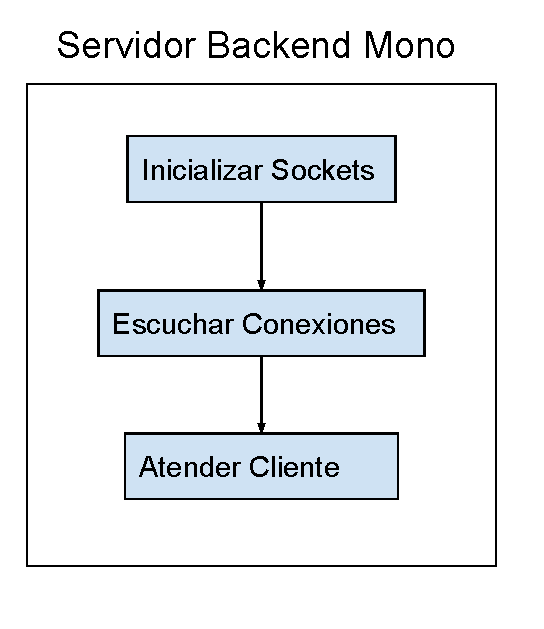
\includegraphics[scale = 0.5]{./imagenes/so_tp2_1.pdf}
	\caption{Diagrama el funcionamiento del backend mono.}
	\label{fig:fig1}
  \end{center}
\end{figure}

\subsection{Backend múltiples clientes}

El cambio más importante para darle soporte multiusuario al backend radica en el uso de threads de la librería \textbf{pthreads}. Inicialmente realizamos las mismas operaciones que el backend mono para setear el tablero y los sockets y luego nos quedamos a la espera de conexiones entrantes. Pero, al momento de recibir una nueva conexión en lugar de derivar todo el flujo de ejecución del programa a la rutina de atención del cliente, creamos un nuevo hilo de ejecución (\textit{thread}) que se encargara de ello con la función \textbf{pthread\_create}. También, mantenemos abierto el socket a la espera de nuevos clientes y tenemos ejecutándose concurrentemente la rutina que acepta a los clientes y las rutinas que atienden a los cliente así puedan conectarse muchos clientes en el juego.

\begin{figure}[H]
  \begin{center}
	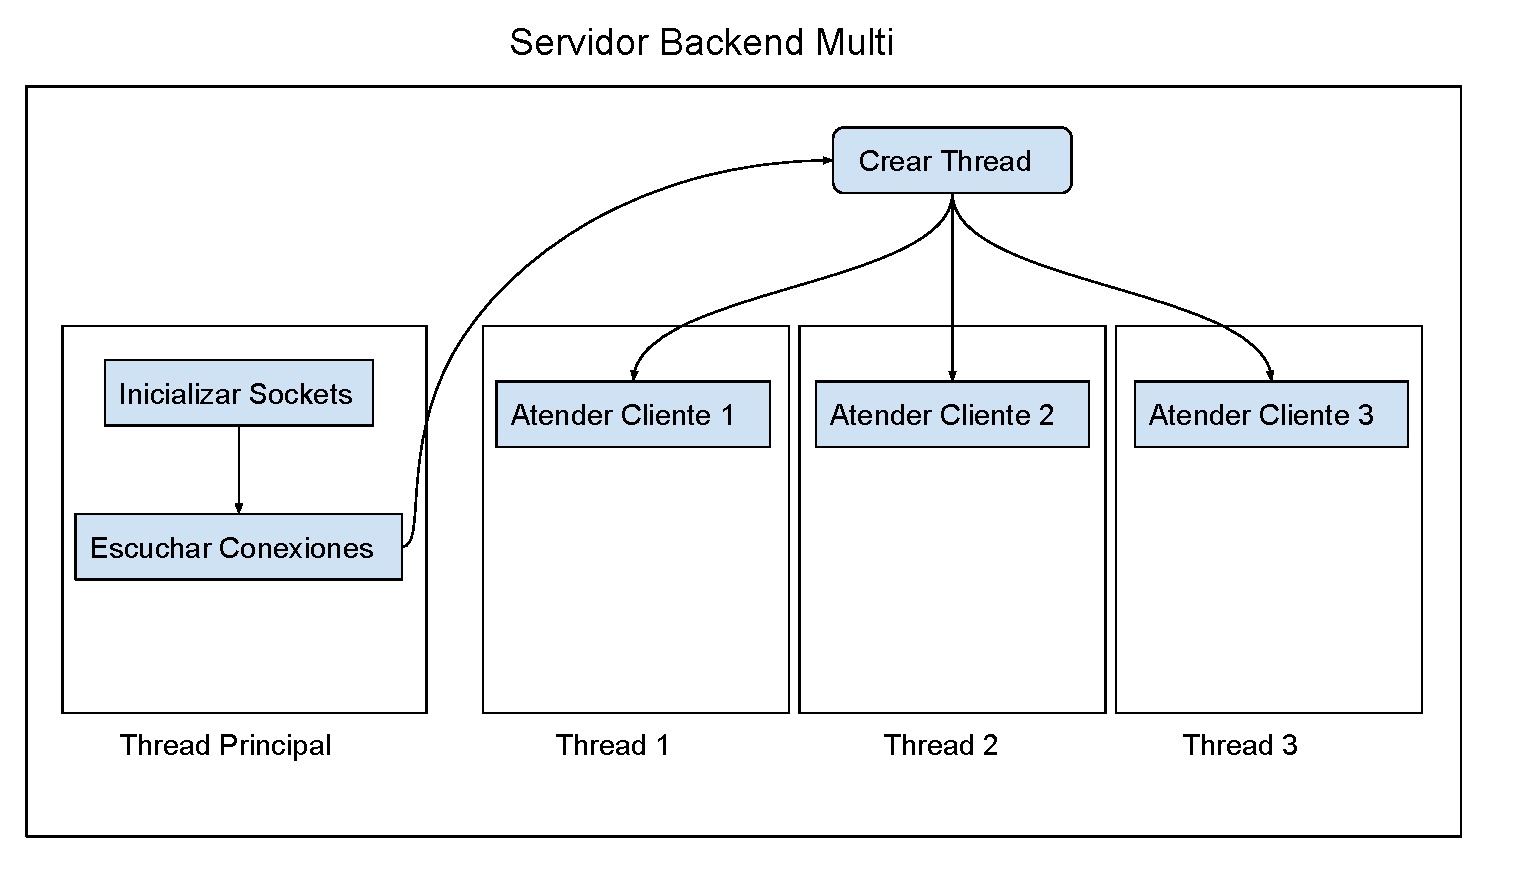
\includegraphics[scale = 0.4]{./imagenes/so_tp2_2.pdf}
	\caption{Diagrama ilustrativo del backend multiusuario}
	\label{fig:fig2}
  \end{center}
\end{figure}

La siguiente cuestión a resolver para mantener la correcta sincronización entre los hilos y estar libres de condiciones de carrera, fue determinar las zonas críticas del servidor. El servidor cuenta con dos variables globales compartidas por todos los threads, estas son \textit{tablero\_temporal} y \textit{tablero\_confirmado}. Estas variables son leídas y escritas con las distintas acciones de los clientes, por lo tanto estas serán nuestras secciones críticas a las cuales debemos garantizar el acceso exclusivo para mantener la coherencia. Esto lo hacemos aprovechando los mecanismos provistos por la clase implementada anteriormente \textbf{RWLock}, así que agregamos dos instancias globales de esta clase, \textit{lock\_tablero\_temporal} y \textit{lock\_tablero\_confirmado} con el fin de garantizar el acceso exclusivo a las secciones críticas. Vamos a listar las funciones del juego con los cambios efectuados:

\begin{itemize}
	\item Atender jugador:
		\begin{itemize}
			\item Colocar una carta: En esta operación estamos modificando el tablero temporal con la carta colocada, solicitamos el \textit{write-lock} del tablero temporal, efectuamos el cambio, y luego lo liberamos \textit{write-unlock}.
			\item Confirmar jugada: Necesitamos escribir en el tablero confirmado la jugada del cliente pedimos \textit{write-lock} en el tablero confirmado por cada escritura realizada de la jugada y al finalizar liberamos \textit{write-unlock}.
		\end{itemize}
	\item Enviar tablero: Enviamos el tablero confirmado a un cliente y para eso leemos el tablero confirmado, así que solicitamos el \textit{read-lock}, efecutamos la lectura y luego hacemos un \textit{read-unlock} 
	\item Quitar cartas: El tablero temporal debe ser limpiado, se debe escribir en todas sus coordenadas, por ello realizamos un \textit{write-lock}, limpiamos la coordenada y luego un \textit{write-unlock}.
	\item Es ficha valida: En esta operación comprobamos si una jugada es válida, para ello debemos leer tanto el tablero temporal como el tablero confirmado, solicitamos con sus respectivas instancias de \textbf{RWLock} el \textit{read-lock} cada vez que el casillero necesite ser leído, luego lo liberamos con \textit{read-unlock}
\end{itemize}

Finalmente, luego de garantizar el acceso exclusivo a las secciones críticas, sólo nos queda finalizar el thread cuando el cliente términe su conexión con el servidor, para ello agregamos en la rutina encargada de terminar el cliente un llamado a \textbf{pthread\_exit} que indica que el hilo actual ha finalizado.

